\chapter{Conceptual Framework}\label{sec:concept}
Based on the preparations in Chapter~\ref{sec:analysis:examples} this chapter specifies a conceptual framework for \cmvs{}.
The approach involves the definition of the terminology, a formalization of an interaction and the basic components of the conceptual framework.
These components are derived from the interactions and the data structures discovered in Chapter~\ref{sec:analysis}.

\section{The Conceptual Framework from the User Perspective}\label{sec:concept:framework}

Figure~\ref{fig:concept:component-diagram} shows a component diagram of the conceptual framework.
The user interacts via input devices, e.g. mouse or keyboard, with a computer.
In order to see the effect of the interaction the user oberserves an output device like a screen.

The computer or the browser provides an \gls{api} for these devices and the implementation of each view has access to this \gls{api}.
On the other side, views can communicate with each other through a coordinator.
This is necessary in order to coordinate interactions.

Each view can have multiple triggers and multiple effects.
A trigger is the handling of an event, caused by a user interaction, e.g.\ a mouse click.
A effect is the change of the visual representation of the view, in order to communicate the interaction.

Each view is self-responsible for the implementation of triggers and effects.
This is inevitable, as sometimes a view can not react to an interaction at all.
E.g.\ a re-ordering in a parallel plot will not affect a scatter plot, where the position of items is contrained by coordinates.

Interactions of the same category also need to be distinguishable.
E.g.\ the user could select a group of items with a bounding box.
Additionally, the user moves the mouse cursor on an item within that group in order to highlight the item.

Therefore the message exchanged between views not only includes the interaction category and the relevant item but also an interaction purpose.

Every view can subscribe to named interactions at the coordinator.
The coordinator notifies all subscribed views when a named interaction happens.
In order trigger an interaction, the visualization simply publishes the named interaction at the coordinator.
This pattern is known as the \emph{Publish-subscribe pattern} and widely used in message queues.


\begin{figure}[ht]
  \centering
  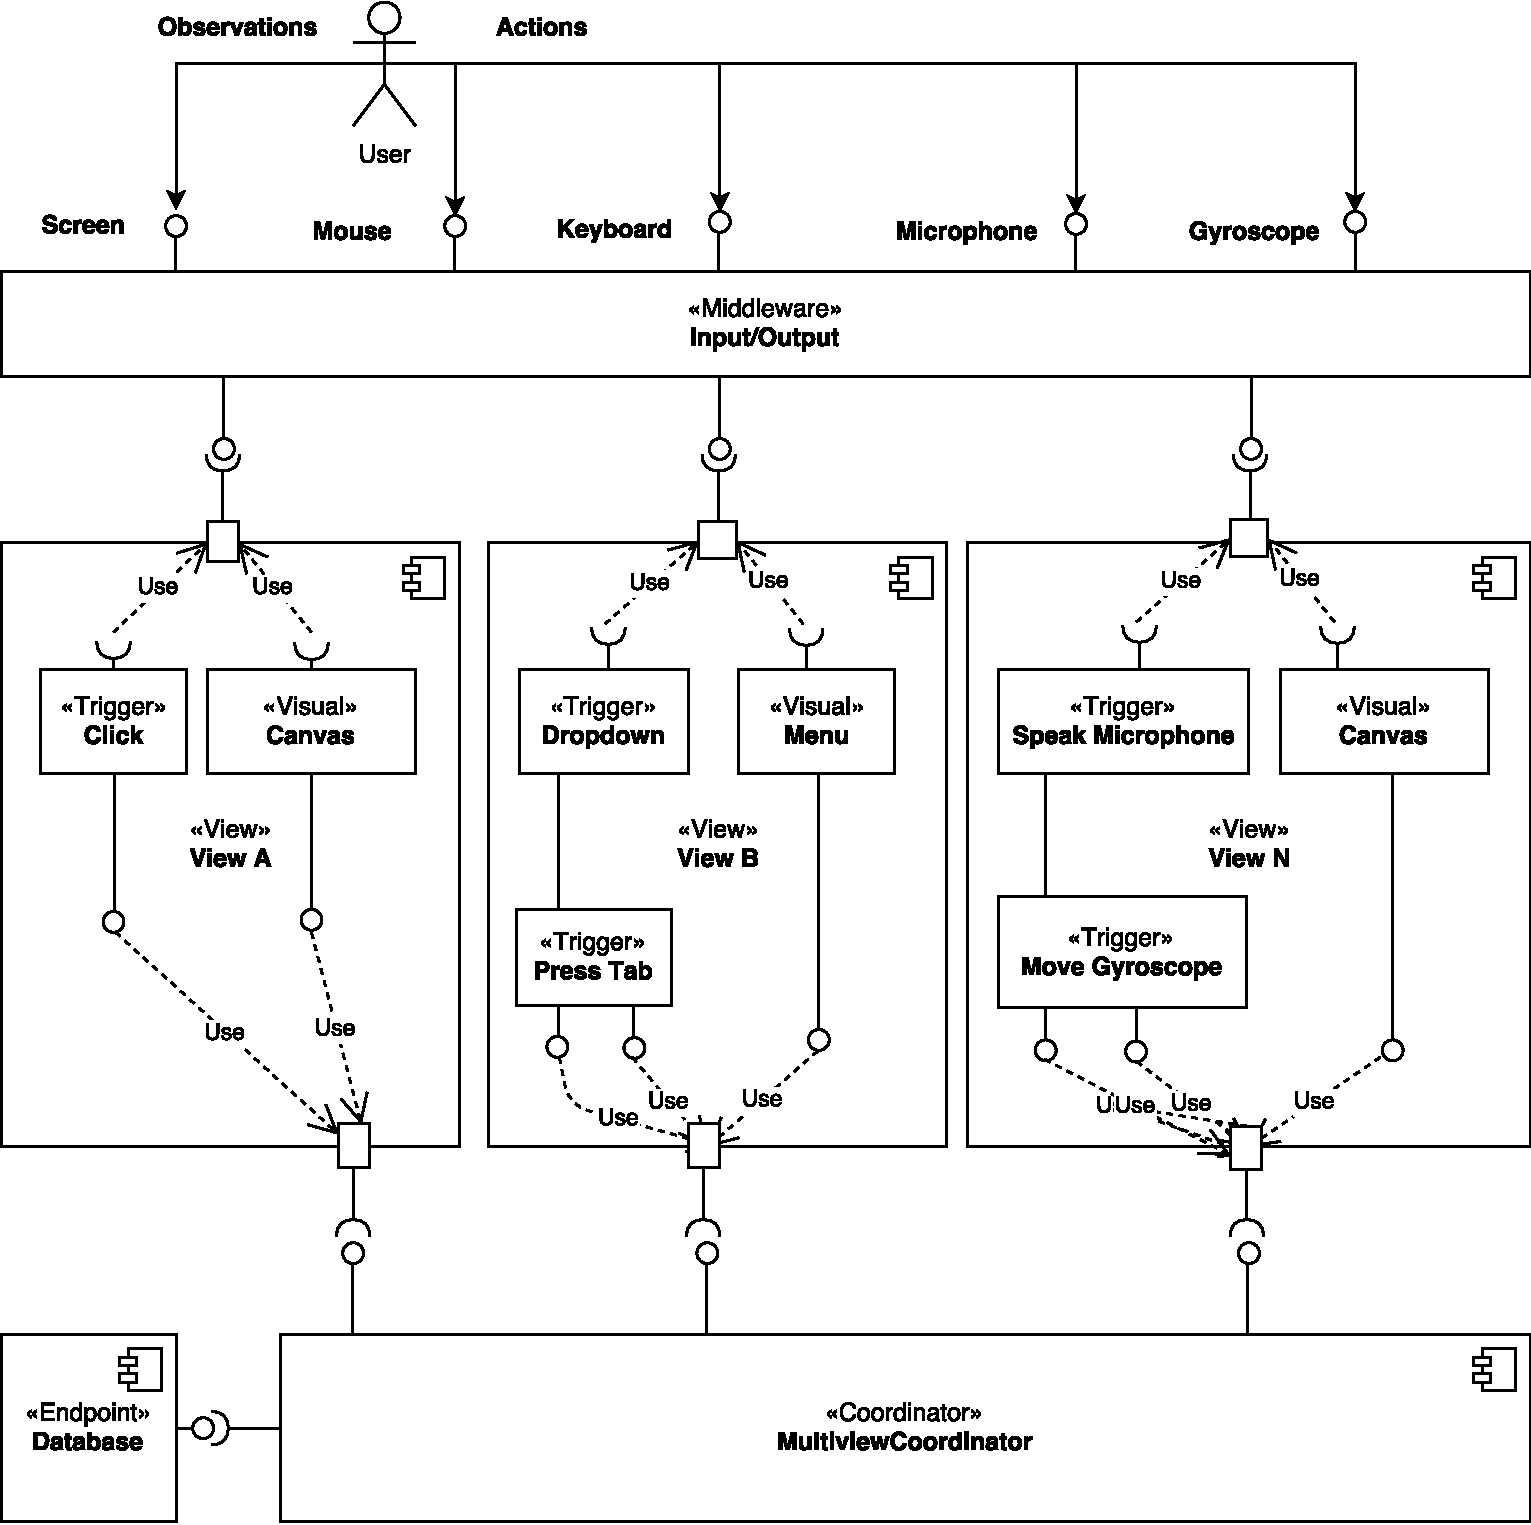
\includegraphics[width=\textwidth]{figures/concept/Concept}
  \caption{%
    Component diagram of the conceptual framework.
  }\label{fig:concept:component-diagram}
\end{figure}


\subsection{Interaction}
In single views, an interaction $I$ consists of at least a trigger and an effect:
\begin{equation}
  I(T, E)
\end{equation}
The purpose of the interaction in a single view does not need to be explicitly stated as such.
E.g.\ hovering over a geographic area changes the background colour of the polygon and the user can identify the interaction as a \emph{highlighting}.
This implicit meaning gets explicit in the described conceptual framework, so that views are able to react reasonably to interactions in other, outside views.

\subsection{Interaction in Coordinated Multiple Views}\label{sec:concept:framework:interaction}
An interaction $I$ in \cmvs{} is formalized as
\begin{equation}
  I(T, M(C,P,S), E)
\end{equation}
for a trigger $T$, a message $M$ and the effect $E$.
The message $M$ is defined by a category $C$, an application specific purpose $P$ as well as an interaction subject $S$.
The shared part of the interaction among multiple views is the message $M$.

\subsection{View}
A view is the section of the screen in which the user can see a data visualization.
A \cmv{} system shows multiple views, either side by side on a single screen or on different screens which are physically placed next to each other.


\subsection{Trigger}
If the event of a user action is handled by a view and causes an interaction, this handling is called a \emph{trigger}.
The user e.g.\ clicks on a shape in the view, hovers over an area, selects an item from a dropdown menu, turns around a mobile device, speaks into the microphone or makes a particular gesture.
As described in the introduction, views are responsible of their \emph{triggers}.


\subsection{Effect}
The effect is the change of the visual representation subsequent to the interaction.
In order to be perceivable by the user, the interaction must have some visual effect, e.g.\ a change of a visual variable according to \textcite{Bertin2010}.

Some examples are:
A change of colour of a selected bubble, a movement of the viewpoint, a rearrangement of attributes in a parallel plot or a higher level of detail in a \tmap{}.

Similar to a \emph{trigger}, a view is self-responsible of its visual \emph{effects}.
Obviously visual effects are not shared, as a visual variable might be constrained due to the nature of the visualization technique itself.
A re-ordering interaction in a parallel plot will not have an effect in bubble charts, as position is constrained by the type of visualization.

\subsection{Category}
An category is the declaration and definition how the subject of the interaction should be changed.
The aforementioned explicit meaning of the interaction is the smallest unit of information of the interaction.
Some examples of categories include: Selection, Deletion, Point-of-Interest, Filtering, Reordering, Re-encoding.
Categories can be classified with the interaction categories of \textcite{Yi2007}.

\subsection{Purpose}
The \emph{purpose} describes the interaction in the context of a task or an application specific intention.
A developer may want to have many \emph{select} interactions.
E.g.\ the user desires to select a detail view of an item under the mouse cursor from a previously selected set of already highlighted items.
Therefore two interactions of the same category can be distinguished by a user-defined \emph{purpose}.

\subsection{Subject}
A subject refers to the target of the interaction.
We must define what data or meta-data is affected by the interaction.
E.g.\ when a user moves the mouse cursor on a line in the line diagram, that could highlight the \emph{data point} under the cursor as well as the entire \emph{data series}.
Therefore we call the object affected of an interaction the interaction \emph{subject}.
A subject can be a data point, a list of data points, a position of the viewpoint, a certain order of attributes or a mapping of attributes to visual variables.



\section{Shared data model}\label{sec:concept:data-model}
The shared data model is a model of the data on which all visualizations must agree on.
To account for various data structures discovered in Chapter~\ref{sec:analysis}, we use an abstract data model that is inclusive enough to include tabular, hierarchical and relational data.
You can see a class diagram of this data model in Figure~\ref{fig:concept:shared-data-model}.

The \emph{entity} class is used to model the smallest distinguishable unit.
All entities can be identified and retrieved via the \emph{id}.
An entity is defined to be any object that can have data attributes attached as \emph{dimensions}.

While entities describe what an object \emph{is}, a \emph{dimension} describes what it \emph{has}.

An entity can have arbitrary many attributes and each value can be accessed by the name of the attribute.
So if you want to get the \emph{latitude} value of an entity, you can retrieve the value with a call to the dimension \emph{latitude}.

Entities can also be \emph{series} of other entities.
A series contains an ordered list of contained entities.
As series can also contain other series, so we can model a hierarchy relation.

Every entity has a \emph{parent} which is the series it is contained in.
The root entity of the hierarchy has a parent which is \attr{nil}.
Every series has a special attribute \attr{height} that describes the number of nested series or the height of the subtree.

If we just want to display tabular data, we just have one or two levels of hierarchy.
E.g.\ one level of hierarchy for a histogram and two levels of hierarchy for a stacked bar chart.

Other relations than hierarchical relations can be modeled as a \emph{relation} entity.
It represents a directed edge in a graph and must have incoming and outgoing entity.
Since every \emph{relation} is an \emph{entity} as well, we can add \emph{attributes} to the relation.
These attributes may describe e.g.\ the weight of an edge in a flow map.

\begin{figure}[ht]
  \centering
  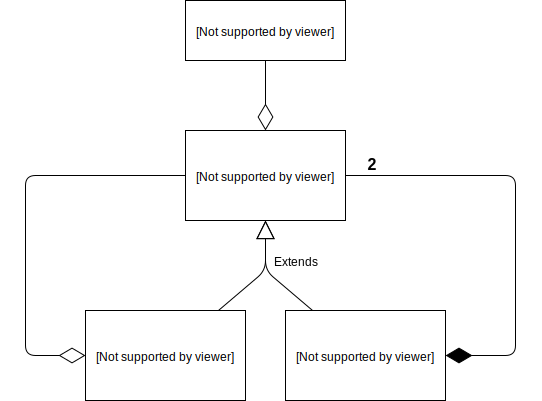
\includegraphics[width=\textwidth]{figures/concept/DataModel}
  \caption{%
    A data structure for tabular, hierarchical and relational data.
  }\label{fig:concept:shared-data-model}
\end{figure}



\section{Encoding of Interaction Subjects}\label{sec:concept:message-interface}

As described in Section~\ref{sec:concept:framework:interaction}, a message consists of the interaction \emph{category}, \emph{purpose} and \emph{subject}.
Category and purpose are just identifiers and can be encoded as a number or a string.
The subject is a highly variable object.
It could define some state, e.g.\ explicitly stating the id of an entity or the name of an attribute.
Alternatively, it could define some behaviour, e.g.\ implicitly defining if an entity is filtered based on its dimensions.
Therefore, the approach in this thesis is to model the subject as a mathematical function.
If the function has no input parameter, it just returns some state, i.e.\ the ids of \emph{entities}, \emph{series}, and \emph{relations} or their respective \emph{attributes}.
If the function depends on input parameters, it may return e.g.\ \attr{true} or \attr{false} or define a sort order.

In this section, a couple of function declarations are derived from the examples in Section~\ref{sec:analysis:examples}.
Domain and range of these functions refer to the objects defined in the data model in Section~\ref{sec:concept:data-model}.

\subsection{Set definitions}
The set of all entities $E$ in our subject space is defined as:
\begin{equation} \mathbb{E} : \mathbb{E} \subseteq \mathbb{N}  \end{equation}
Each entity can be represented by its \attr{id}, so for simplicity $\mathbb{E}$ is a subset all natural numbers in $\mathbb{N}$.

The set of all dimensions $D$ in our shared data model is defined as:
\begin{equation} \mathbb{D} : \mathbb{D} \subseteq \Sigma^* \end{equation}
For simplicity, each dimension is represented as a sequence of characters, with the set of all sequences of characters written as $ \Sigma^*$.

The set of all values of a dimension $d$ is defined as:
\begin{equation} Space(d), d \in \mathbb{D} \end{equation}
So for an attribute \attr{name}, $Space(name)$ would be the set of all strings.

Visual variables according to \textcite{Bertin2010} as in in Section~\ref{sec:related-work:visual-variables} are defined as:
\begin{equation} \mathbb{V} = \{position, size, shape, value, hue, orientation, texture\} \end{equation}


\subsection{Function declarations}
The functions $Select$ and $Filter$ operate on entities and can be used interchangeably:
\begin{equation} Select: \varnothing \rightarrow \mathcal{P}(\mathbb{E}) \end{equation}
\begin{equation} Filter: \mathbb{E} \rightarrow \{ \bot, \top \} \end{equation}
  Its domain is the empty set $\varnothing$ and the set of all subsets of $E$ is written as $ \mathcal{P}(\mathbb{E})$.

  $Select$ just returns a subset of entities explicitly and expects no input.
  It can be used to highlight or focus entities, mark them for deletion or show details of an entity.

  $Filter$ returns for every entity either \attr{true} or \attr{false}, depending on the entity and the value of its dimensions.
  Instead of an explicitly defined set of filtered entities, entities are defined implicitly.
  A good example would be a filter function checking upper and lower limit for each entity and a dimension called \attr{price}.

\begin{equation} Window: \mathbb{D} \rightarrow W, W = \{w | w \subseteq Space(d), d \in \mathbb{D}\} \end{equation}
  For each of the dimensions in $\mathbb{D}$, the function returns the currently visible subset.
  E.g.\ a zooming or panning operation in a \gv{} would result in a change of \attr{latitude}, \attr{longitude} and \attr{zoom} of the viewpoint and therefore the currently visible section of the geographic vector space.
  The subset $w$ can be encoded implicitly or explicitly.
  For continuous values two representatives \attr{from} and \attr{to} could define an interval.
  E.g.\ in a calendar we map \attr{fromDay}, \attr{toDay}, \attr{fromHour} and \attr{toHour} to define the currently visible time section.
  If a dimension has discrete values, subset $w$ could also be encoded with all values explicitly stated.

\begin{equation} Order: \mathbb{E} \times \mathbb{E} \rightarrow \mathbb{R} \end{equation}
  The $Order$ function is used to order two arbitrary entities $e1, e2 \in \mathbb{E}$.
  If $e1 < e2$ then the return value $r$ will be $ r < 0 $.
  For $e1 = e2$ the statement $r = 0$ holds and for $e1 > e2$ then $r > 0$.

  Similar to $Filter$, the $Order$ function can either be implemented explicity or implicitly.
  An explicit implementation returns a value $r$ based on the relative position of $e1$ to $e1$ in a given sequence.
  An implicit implementation would return a value $r$ based on some computation of dimensions of $e1$ and $e2$.
  E.g.\ ordering entities based on the alphabetical order of their name would be an example of the latter.

\begin{equation} Encode: \mathbb{D} \rightarrow \mathbb{V} \end{equation}
  The $Encode$ function can be used to change any mapping of dimension to any visual variable.
  E.g.\ bar charts, line diagrams, histograms and bubble charts can change the attribute mapped to the \attr{y} and \attr{x} axes.
  Bubble charts can encode a different dimension in the \attr{size} of the bubbles.
  Choropleth maps, treemaps and bubble charts can map a different attribute to the \attr{colour}.
  A specialized version of this function may return the attribute that is used for the \attr{layout} of the tiling algorithm in treemaps.
  Note that parallel plots have arbitrary many \attr{y} axes.
  To define the order of dimensions displayed in a parallel plot, each dimension will be mapped to a named \attr{y} axis, e.g. $y1, y2 ... y3$ and so on.

Let's have some examples how these functions can be applied on coordinated interactions:

A user clicks on a bar in a bar chart and this feature then changes its background colour.
To coordinate the highlighting, the bar chart view will formulate a new message composed of a \emph{Select} function and the category \emph{highlight}.
The function returns the set with the highlighted entity.

Let's say, a geographical map should move the position of the viewpoint on a entity.
The triggering view will use a function \emph{Select} this time with a category \emph{focus}.
A treemap as a third view could pick up that interaction and show a subtree with the focused entity as root node. 

A view may show some controls to filter the data set, e.g.\ two sliders on an attribute called \attr{prize}.
When the user releases the mouse, an interaction with the function \emph{Filter} and the category \emph{Hide} will be triggered.  
The function will then check the \attr{prize} of every entity and returns \attr{true} if the prize is within the given lower and upper limit, \attr{false} otherwise.


